\section{Introduction}\label{sec:intro}

%After generations of technological revolutions, from wired to wireless
%communications, stationary to mobile machines, and large-sized to hand-held
%devices, we are now witnessing what can be deemed as the next phase of mobile
%technology: widespread {\em wearable computers}.
%Research in wearable computers can be dated back at least to the 1980s when
%Steve Mann experimented with backpack computers and developed a prototype of
%heads-up-display goggles~\cite{mann1997wearable}.
%Wearable devices have become pervasively available and are on the way to become an integral part of human
%lives~\cite{googleglass,smartwatch,fitbit}.  %This is thanks to the advances in hardware miniaturization technology, affordable
%sensors and processor chips, and low-power computing.
%In this paper we focus on special-purpose wearable devices that are worn close
%to the body as opposed to the more general-purpose computing/communication
%platform like smartphones or tablets. Examples are smart glasses, smart
%wristbands, and smart watches, smart jewelry, and devices embedded in clothing
%like jackets or shoes. Such devices are typically very small and impose severe
%resource constraints.
%This is clearly evident from the surge in the number and types of wearables
%that are commercially available -- ranging from smart glasses, smart
%necklaces, smart wristbands, to smart watches.
%With the proliferation of such wearable devices, they can be expected to be subjected to malicious attacks and preserving the security and privacy of these devices will become increasingly important.
Wearable devices are on the way to become an integral part of people's daily lives~\cite{googleglass,smartwatch,fitbit}.
These devices collected data about the wearers, their surroundings and often even about their health.
It is thus critical to the users' privacy, that this data is protected from unauthorized access. Although there has been work~\cite{hoyle2015sensitive,hoyle2014privacy,jana2013scanner} on limiting privacy
threats from ubiquitous photography enabled by the wearable devices, robust usable and secure authentication systems
leveraging the devices have not emerged.
%however, to the best of our knowledge we are the first to address user
%authentication directly with these devices.
An authentication system for these devices has to strike an
appropriate balance with user convenience, especially since users are interacting
with an increasing number of wearables. %A fundamental building
%block for securing wearable devices and their data is efficient user authentication. %, since many
%solutions are only effective as long as the device itself is authenticated to
%the right user/owner.
%In this paper, we thus focus on wearable device authentication techniques that are both efficient and convenient.

\vspace{1mm}\noindent{\bf Authentication Challenge.}
%User-authentication for wearable devices has so-far received relatively less
%attention; commercially as well as in research.
Today, authentication on most commercially available wearable devices~\cite{fitbit, smartwatch} relies on an indirect mechanism, where users
can log in to their wearables through phones. This requires the wearable
device to be registered and paired to the mobile device, and both devices to be carried by the user, which can be highly inconvenient in reality. The security of this
approach is also in question as it increases the chance of hacking into both
devices if either is lost or stolen. Some devices including
Google Glass~\cite{googleglass} and FitBit's health tracker~\cite{fitbit}
allow linking the device to online accounts instead of a mobile device for
convenience,  which, however, does not add to security. Indirect authentication
remains a
dominant paradigm for wearables despite these fundamental shortcomings because
such devices are \emph{seriously resource-constrained} in many aspects:
battery power, computational and storage capabilities, and input/output. As a result, typical authentication methods designed for more
powerful devices can not be directly applied here; rather, user authentication for wearable devices must operate indirectly
through a more capable device. We, however, take the viewpoint that wearables will become more independent
units that have to maintain security guarantees without such paired devices
and we seek to develop suitable \emph{direct authentication} methods that are
both accurate and light-weight.
\vspace{-1mm}
\begin{figure}[t!]
\centering
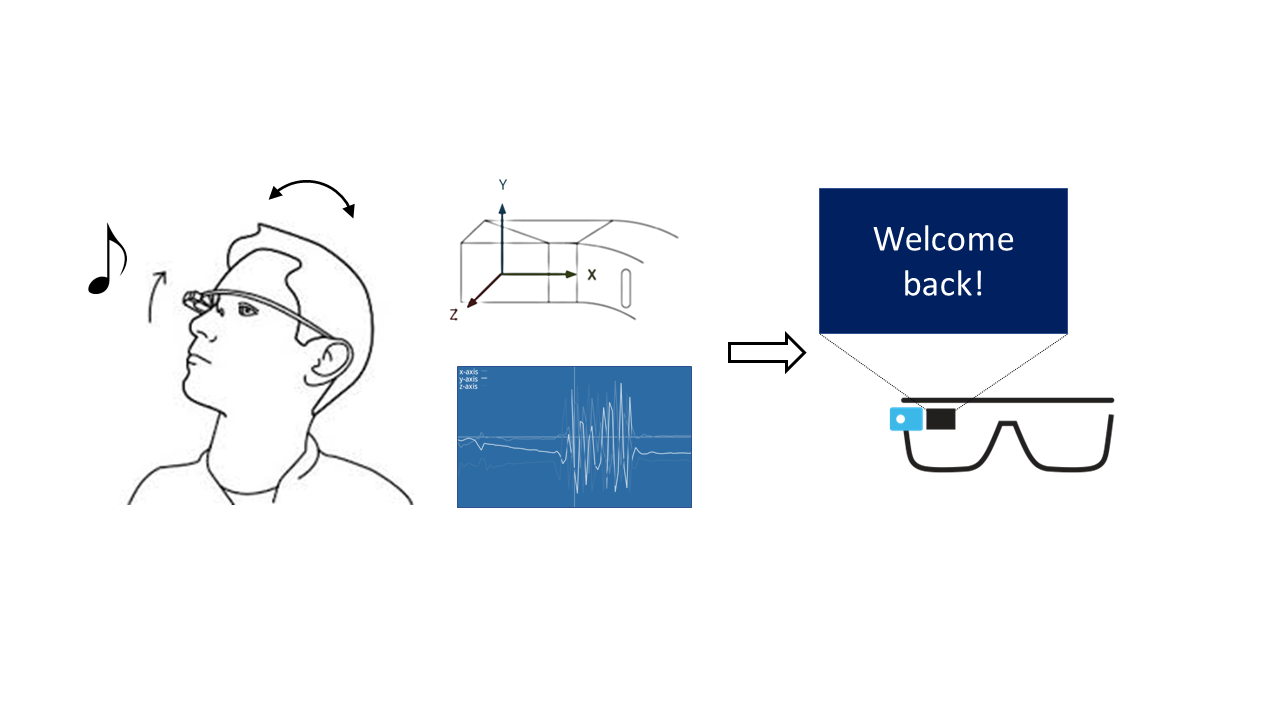
\includegraphics[width=\columnwidth]{figure/headbanger_illustrate.png}
\caption{Illustration of Headbanger. The head-worn device authenticates the
users based on signatures generated from head-movement patterns.  These patterns are created in
response to an audio snapshot played on the device.}
\label{fig:headbanger-illustrate}
\end{figure}

%For example, fitness trackers and
%smart-watches are tethered to user's mobile device to connect to the
%Internet as well as for remote data collection.
Before we explore direct authentication methods for wearable devices, let us
first consider available solutions for other mobile systems, especially
smartphones and tablets. Broadly speaking, the two most commonly used
authentication methods on mobile systems are (arguably) password-based methods
(with their variants) and biometric-based methods. However, we argue that
neither of these two methods is really suitable for wearable devices. Typing
passwords or drawing swipe patterns on wearable devices can be quite
cumbersome due to their small input/output units, if they do have a touch
sensor at all. Collecting and recognizing physiological biometrics (such as
DNA, fingerprint, hand/finger geometry, iris, odor, palm-print, retinal scan,
voice, etc.) requires specialized sensing hardware and processing resources
that add cost, and many of these sensors are even larger than the size of wearables
themselves.

We therefore focus on a third class of direct authentication methods: relying upon the uniqueness of human behavior characteristics such as human walking gait, arm swings, typing patterns, body pulse beats, eye-blinks, etc. This way of authenticating users is often referred to as behavior-based authentication, and it has been studied in the context of authenticating smart phones and tablets~\cite{rahman2014bodybeat,cornelius2014wearable,stevenage1999visual,okumura2006study,monrose2000keystroke,jorgensen2011mouse,bo2013silentsense,de2012touch}. The main advantage of using behavioral characteristics for mobile device user authentication is that the signatures can be readily generated from raw data of built in sensors such as motion sensors, camera, microphones etc. Considering that cameras and microphones, as well as vision and audio processing algorithms, are quite energy-hungry, we thus focus on those behavioral characteristics that can be easily captured by sensors that require less power consumption, such as accelerometer. More specifically, we propose to authenticate wearable devices to users based on the following behavioral characteristic: our unique body movement patterns and their dependence on external stimuli that wearable devices can generate, such as vibrations and music.

\vspace{1mm}\noindent{\bf Head-movement based authentication.} Body movement
patterns have long been used by humans to discriminate between people. By
watching how a person walks, dances, waves hands, we can often recognize
the person from afar. This is because human body movements are usually
\emph{distinctive} and \emph{repeatable}. Achieving the same through
wearables, however, is not straightforward and poses significant research
challenges: it is unclear whether these seriously-constrained devices are able
to capture the differentiating characteristics of movement patterns, process the data, and quantify the
uniqueness of each user's behaviors. Moreover, each device will have only a
limited view of body movements, dependent on its mounting position on the
human body. In this paper, we set out to conduct a holistic study of wearable
authentication through body movements and to design an \emph{accurate, robust,
light-weight, and convenient} authentication system. A key distinguishing feature of our work
is that we will also consider stimuli that wearable devices can provide to
design challenge-response inspired mechanisms, particularly stimuli that are
difficult to observe even for the closest adversaries. For example, we can use
fast-tempo music through earbuds to stimulate movements and to make such
free-style movements more repeatable.

In particular, we have designed, implemented and evaluated {\em Headbanger},
an authentication system that can authenticate users by motion sensing head movement when listening to music beats. Although we
use Google Glass as a running example, our design can
be applied to other head-worn gadgets and any system that can record
head-movements through motion sensing. Our choice for using head movements is
motivated by the fact that head-worn wearables are becoming very common today
and such devices are already equipped with motion sensors; for example,
personal imaging and heads-up display devices, gaming headsets, augmented reality devices.

%Unlike physiological biometrics that require custom hardware,
%behavioral biometrics offer a much more available/conveient solution. The
%challenge, however,
%is to ensure that these patterns are repeatable under all circumstances that
%the user encounters as well as the differentiability factor between different
%human beings. %We show that by using the same external stimulus among all
%%users
%the baseline for comparison is achieved much easier and the head-patterns are
%more consistent and differentiable among users.

%Subconscious head-movement, or any body movement as a matter
%of fact, can be very random in general.
% Our design assumes that there is only one owner per glass, and we can easily
%extend our scheme to handle the cases with multiple owners.

In summary, the key contributions of this paper are:

\begin{enumerate}

\item We have designed and implemented a novel user authentication method for wearable devices
using head-movement patterns. Our study shows that user's head-movement patterns
contain unique signatures that when inferred correctly can be used as valid
means for authentication. We design a system, \systemname, that records, processes, and classifies
head-movement patterns of users based on accelerometer sensor readings.

%\item We devise of a set of light-weight preprocessing and classification
%algorithms that can effectively transform raw and noisy sensor data into
%accurate authentication results. We aggressively optimize the processing
%latencies of these algorithms so that they are well suited for wearable
%devices.

\item %We implement a data collection application on Google Glass that plays a
%fast beat music (preloaded) through the Glass's speakers and simultaneously
%records and filters accelerometer sensor data. We use this data collection app
%in our experiments to evaluate the system.
Through comprehensive experiments
involving 95 users and over
different system design parameters we show that head-movement patterns
can generate accurate authentication results. Our approach effectively identifies a wearable device user, with an average false
acceptance rate of 4.43\% and an average true-positive rate of 95.57\%. Also, we show that our authentication method is quite robust: when a user slightly increases her head-movement complexity, it quickly becomes \emph{much harder} for attackers to imitate the movement pattern.


%average false rejection rate of 4.9\%.

\item We implement \systemname~on Google Glass and carefully profile the
execution time of each software module in the implementation. We measure an average processing latency of 1.93 seconds on the Google Glass for the best authentication performance.

%\item We have conducted detailed validation of using head-movement patterns
%as a biometric characteristic by collecting and analyzing data from multiple
%users. We will make these data publicly available, which may facilitate other
%user behavior studies.
\end{enumerate}

%In the sections to follow, we will discuss the background of wearable
%device authentication in section~\ref{sec:background} and details of our
%proposed system design in section~\ref{sec:design}. We evaluate the system in
%section~\ref{sec:results} and follow up with discussions and conclusions in
%sections~\ref{sec:disc} and~\ref{sec:conc}, respectively.












\iffalse
Wearable devices are typically user-interface constrained
Unlike a smartphone, touch gestures or voice activation or face
recognition units not all wearable devices today have the generic
user interfaces such as touch or audio or visual so that typical
gesture or

The recent years have seen a significant growth in popularity of
smart wearable devices. This growth can be attributed to the advances in
hardware miniaturization technology as well as economically affordable
and energy efficient sensing and computing. While size, energy and cost
constraints remain key motives for improvements in wearable computers'
design, the aspect of user authentication has received relatively less
attention. Wearable devices often collect and store sensitive data about
users, and thus there is an obvious need to authenticate the right user to the
device. Solutions today primarily rely on indirect authentication
mechanisms through the user's smartphone, which can be cumbersome and less
secure. Biometric based solutions, though very effective, however, are subject
to the availability of the specific sensors in the wearable unit. In this
paper, we propose to authenticate wearable devices to users based on their
unique behavioral patterns. In particular, we prototype an authentication
system for wearable devices by monitoring user's unique head-movement patterns
in response to an external audio stimulus. Using a personal imaging device as
a running example, and through extensive experimental evaluation over multiple
users, we show that our mechanism can authenticate users with high accuracy


\fi 